\documentclass[a4paper,10pt]{article}

\usepackage[T1]{fontenc}
\usepackage[french]{babel} 
\usepackage{lmodern}
\usepackage{graphicx}
\usepackage[utf8]{inputenc}

\title{Guide d'utilisation de 3DSolve}
\author{Lisa Aubry, Alban Chazot, Korlan Colas, Anthony Gourd}
\date{\today}

\pdfinfo{
  /Title    (Guide d'utilisation de l'application 3DSolve)
  /Author   (Lisa Aubry, Alban Chazot, Korlan Colas, Anthony Gourd)
  /Creator  (Lisa Aubry, Alban Chazot, Korlan Colas, Anthony Gourd)
  /Producer (Lisa Aubry, Alban Chazot, Korlan Colas, Anthony Gourd)
  /Subject  (Application ``SolidSnake''; résolution du algorithmique du casse-tête ``Snake Cube'')
  /Keywords ()
}
\begin{document}
\maketitle

Ce document vise à décrire rapidement et efficacement les méthodes d'utilisation de l'application 3DSolve.

\section{Utilisation en ligne de commande}
L'application propose quelques options en ligne de commande.

\paragraph{--snake} [chemin] permet de charger un snake autre que celui par défaut au démarrage du programme. A noter qu'il est possible de charger d'autre snake une fois le programme démarré (voir plus loin).

\paragraph{--threadNb} [nombre max de thread] permet d'indiquer le nombre maximal de thread que vous souhaitez que l'application utilise pour chercher les solutions. Par défaut le nombre de thread utilisés est égale au nombre de points de départ pour le snake sélectionné.

\paragraph{--help} pour avoir l'aide.

\newpage
\section{L'interface}
Dans cette section, nous allons détailler la composition de l'interface de l'application. La figure~\ref{guide} explicite les différentes composantes de l'application.

\subsection{Le menu}
Le menu de l'application comporte trois sous-menus :
\begin{itemize}
 \item Le sous-menu ``App'' qui donne ensuite la possibilité à l'utilisateur de quitter l'application, de revenir à l'écran d'accueil, d'afficher la page d'aide ou encore la page ``A propos'';
 \item Le sous-menu ``Load Snake'' qui permet de charger et de résoudre un autre serpent;
 \item Le sous-menu ``Solution'' qui permet de sélectionner parmi les différentes solutions possibles celle que l'on veut visionner.
\end{itemize}

\subsection{Le casse-tête}
Le casse-tête à proprement parler est affiché au centre de l'écran. Il est possible d'interagir avec lui, autrement-dit, d'effectuer des rotations. Pour cela il faut :
\begin{enumerate}
 \item Sélectionner le cube à faire tourner en cliquant dessus à l'aide du clique gauche de la sourie;
 \item Faire tourner le cube sélectionné en cliquant une nouvelle fois dessus (sans relâcher le clique) puis en déplaçant la sourie dans la direction souhaitée;
 \item Relâcher le clique afin de valider la rotation.
\end{enumerate}

Il est également possible de faire tourner la caméra autour du casse-tête afin d'avoir un meilleur angle de vue. Pour cela, maintenez enfoncé le bouton droit de la sourie puis déplacez la sourie afin de faire se déplacer la caméra en conséquence.

Enfin, vous pouvez également translater la caméra en observant un protocole similaire au précédent. Il vous suffi de maintenir pressé le clique de la molette au lieu du clique droit.

\subsection{Le volume final}
Présent en haut à droite de l'interface, le volume final vous permet d'avoir une idée de la forme à obtenir pour résoudre le casse-tête.

\subsection{Le serpent déplié}
Le serpent déplié représente le casse-tête dans son état initial. Il vous permettra, lors du visionnage d'une solution par exemple, de pouvoir vous ``repérer''. En effet, lorsque vous sélectionnez un cube ou que le visionnage de la solution avance, le cube sélectionné respectivement le cube que la solution vient de traiter ``clignote'' et dans le casse-tête et dans cette représentation dépliée afin qu'il soit facilement identifiable.

\subsection{Flèches de déplacement}
Les flèches de déplacement vous permettent :
\begin{itemize}
 \item En mode solution : d'avancer ou de reculer d'une étape dans le visionnage de la solution
 \item En mode jeu : la flèche de droite vous permet de demander à l'application de vous fournir une aide pour le mouvement suivant. La flèche de gauche vous permet de défaire votre dernier mouvement.
\end{itemize}

Dans un cas comme dans l'autre, ces flèches fonctionnent par simple clique. A noter que vous pouvez également utiliser les flèches directionnelles gauche et droite du clavier pour effectuer les mêmes actions.

\begin{figure}[h]
 \centering
 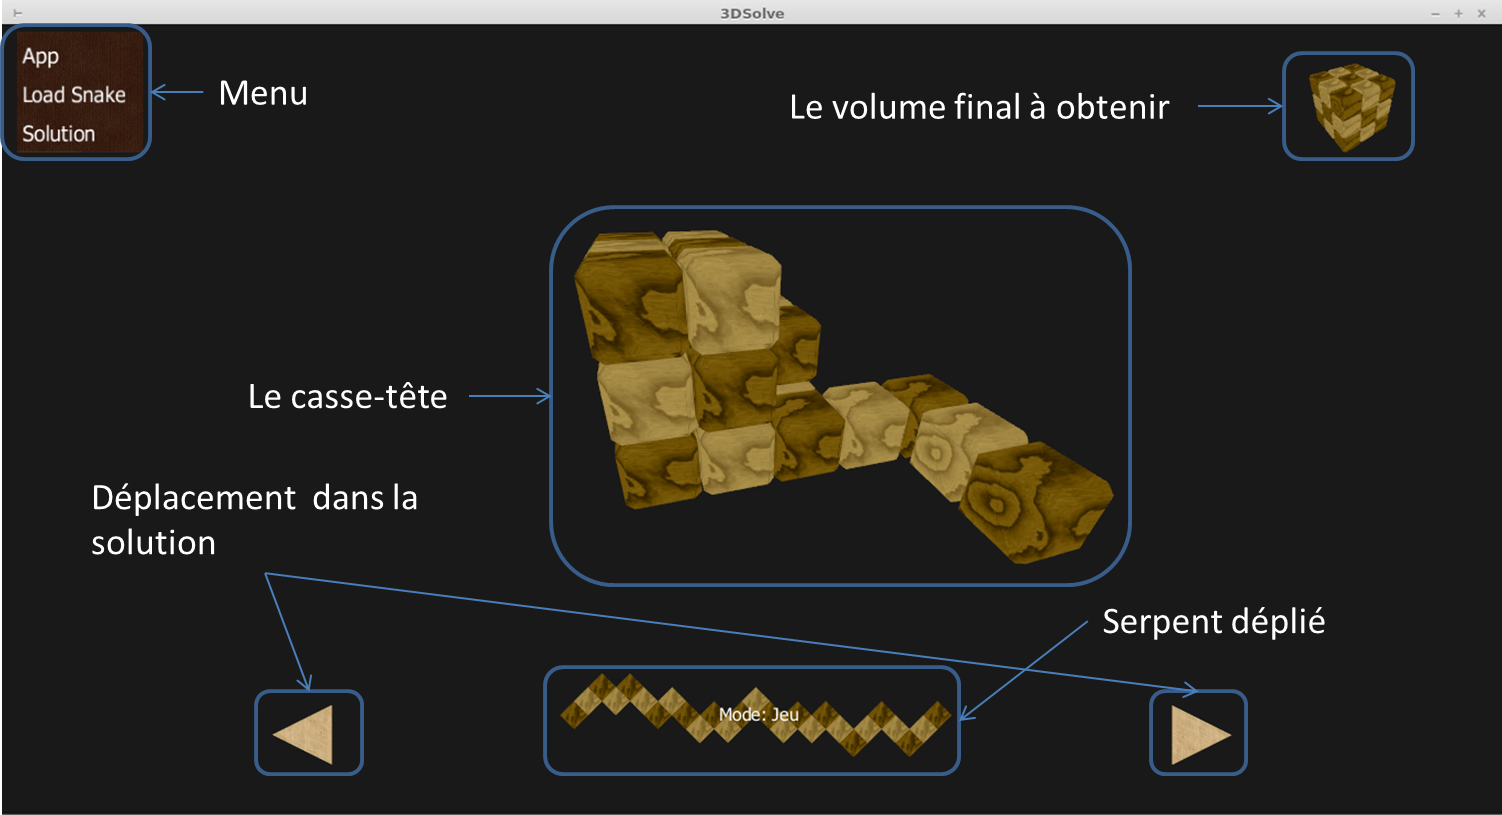
\includegraphics[scale=0.4,keepaspectratio=true]{guide.png}
 \caption{L'interface de l'application}
 \label{guide}
\end{figure}

\subsection{Raccourcis clavier}
3DSolve peut également s'utiliser au clavier :
\begin{itemize}
 \item La flèche directionnelle haut vous permet de ré-initialiser le serpent;
 \item La flèche directionnelle bas vous permet de passer du mode jeu au mode solution et vice-versa;
 \item La touche Espace vous permet d'activer ou de désactiver la rotation du casse-tête autour de lui-mêmes;
 \item La touche Entrée vous permet d'avoir une vision ``éclatée'' du casse-tête et de pouvoir visualiser les liaisons entre les cubes;
 \item La touche F8 (maintenue enfoncée) vous permet de n'afficher que les liaisons entre les cubes;
 \item La touche F9 (maintenue enfoncée) vous permet d'afficher le rendu du color-picking;
 \item La touche échappe vous permet de quitter l'application.
\end{itemize}

\end{document}
